%********************************************************************
% Appendix
%*******************************************************
% If problems with the headers: get headings in appendix etc. right
%\markboth{\spacedlowsmallcaps{Appendix}}{\spacedlowsmallcaps{Appendix}}

%********************************************************************
% Summary of the various Boolean properties and functions (from Chapter 3)
%*******************************************************
\chapter{Boolean Properties and Functions}
\label{ap:ch:boolean_properties_and_functions}

\begin{tabular}{ccc}

	% AND Truth Table
	\begin{tabular}{ccc} 
		\multicolumn{3}{c}{\emph{AND Truth Table}} \\
		\multicolumn{2}{c}{Inputs} & {Output} \\
		A & B & Y \\
		\hline
		0 & 0 & 0 \\
		0 & 1 & 0 \\
		1 & 0 & 0 \\
		1 & 1 & 1 
	\end{tabular}
&
	% OR Truth Table
	\begin{tabular}{ccc} 
		\multicolumn{3}{c}{\emph{OR Truth Table}} \\
		\multicolumn{2}{c}{Inputs} & {Output} \\
		A & B & Y \\
		\hline
		0 & 0 & 0 \\
		0 & 1 & 1 \\
		1 & 0 & 1 \\
		1 & 1 & 1 
	\end{tabular}
&
	% XOR Truth Table
	\begin{tabular}{ccc} 
		\multicolumn{3}{c}{\emph{XOR Truth Table}} \\
		\multicolumn{2}{c}{Inputs} & {Output} \\
		A & B & Y \\
		\hline
		0 & 0 & 0 \\
		0 & 1 & 1 \\
		1 & 0 & 1 \\
		1 & 1 & 0 
	\end{tabular}
\\
\\
	% NAND Truth Table
	\begin{tabular}{ccc} 
		\multicolumn{3}{c}{\emph{NAND Truth Table}} \\
		\multicolumn{2}{c}{Inputs} & {Output} \\
		A & B & Y \\
		\hline
		0 & 0 & 1 \\
		0 & 1 & 1 \\
		1 & 0 & 1 \\
		1 & 1 & 0 
	\end{tabular}
&
	% NOR Truth Table
	\begin{tabular}{ccc} 
		\multicolumn{3}{c}{\emph{NOR Truth Table}} \\
		\multicolumn{2}{c}{Inputs} & {Output} \\
		A & B & Y \\
		\hline
		0 & 0 & 1 \\
		0 & 1 & 0 \\
		1 & 0 & 0 \\
		1 & 1 & 0 
	\end{tabular}
&
	% XNOR Truth Table
	\begin{tabular}{ccc} 
		\multicolumn{3}{c}{\emph{XNOR Truth Table}} \\
		\multicolumn{2}{c}{Inputs} & {Output} \\
		A & B & Y \\
		\hline
		0 & 0 & 1 \\
		0 & 1 & 0 \\
		1 & 0 & 0 \\
		1 & 1 & 1 
	\end{tabular}
\\
\\
	% NOT Truth Table
	\begin{tabular}{ccc} 
		\multicolumn{3}{c}{\emph{NOT Truth Table}} \\
		Input & Output \\
		\hline
		0 & 1 \\
		1 & 0 \\
	\end{tabular}
&
	% Buffer Truth Table
	\begin{tabular}{ccc} 
		\multicolumn{3}{c}{\emph{Buffer Truth Table}} \\
		{Input} & {Output} \\
		\hline
		0 & 0 \\
		1 & 1 
	\end{tabular}
&
\end{tabular}

\hrulefill

%******************************************************
% Univariate Properties
%******************************************************
\begin{table}[ht]
	\caption{Univariate Properties}
	\label{ap:tab:univeriate_properties}
	\sffamily
	\newcommand{\head}[1]{\textcolor{white}{\textbf{#1}}}		
	\begin{center}
		\rowcolors{2}{gray!10}{white} % Color every other line a light gray
		\begin{tabular}{ccc} 
			\rowcolor{black!75}
			{\head{Property}} & \head{OR} & \head{AND} \\
			Identity & $ A + 0 = A $ & $ 1A = A $ \\
			Idempotence & $ A + A = A $ & $ AA = A $ \\
			Annihilator & $ A + 1 = 1 $ & $ 0A = 0 $ \\
			Complement & $ A + A' = 1 $ & $ AA' = 0 $ \\
			Involution & \multicolumn{2}{c}{$ (A')' = A $} 
		\end{tabular}
	\end{center}
\end{table}

%******************************************************
% Multivariate Properties
%******************************************************
\begin{table}[ht]
	\caption{Multivariate Properties}
	\label{ap:tab:multivariate_properties}
	\sffamily
	\newcommand{\head}[1]{\textcolor{white}{\textbf{#1}}}		
	\begin{center}
		\rowcolors{2}{gray!10}{white} % Color every other line a light gray
		\begin{tabular}{ccc} 
			\rowcolor{black!75}
			{\head{Property}} & \head{OR} & \head{AND} \\
			Commutative & $ A + B = B + A $ & $ AB = BA $ \\
			Associative & $ (A + B) + C = A + (B + C) $ & $ (AB)C = A(BC) $ \\
			Distributive & $ A + (BC) = (A+B)(A+C) $ & $ A(B+C) = AB + AC $ \\
			Absorption & $ A + AB = A $ & $ A(A+B) = A $ \\
			DeMorgan & $ \overline{A+B}=\overline{A}\,\overline{B} $ 
				& $ \overline{AB}=\overline{A}+\overline{B} $ \\
			Adjacency & \multicolumn{2}{c}{$ AB + AB' = A $} 
		\end{tabular}
	\end{center}
\end{table}

\begin{table}[ht]
	\caption{Boolean Functions}
	\label{ap:tab:boolean_functions}
	\sffamily
	\newcommand{\head}[1]{\textcolor{white}{\textbf{#1}}}		
	\begin{center}
		\rowcolors{2}{gray!10}{white} % Color every other line a light gray
		\begin{tabular}{llllll}
			\textbf{A} & 0 & 0 & 1 & 1 &  \\ 
			\textbf{B} & 0 & 1 & 0 & 1 &  \\ \hline
			$ F_{0} $ & 0 & 0 & 0 & 0 
			& Zero or Clear. Always zero (Annihilation) \\ 
			$ F_{1} $ & 0 & 0 & 0 & 1 
			& Logical AND: $ A * B $  \\ 
			$ F_{2} $ & 0 & 0 & 1 & 0 
			& Inhibition: $ AB' $ or $ A>B $ \\ 
			$ F_{3} $ & 0 & 0 & 1 & 1 
			& Transfer A to Output, Ignore B \\ 
			$ F_{4} $ & 0 & 1 & 0 & 0 
			& Inhibition: $ A'B $ or $ B>A $ \\ 
			$ F_{5} $ & 0 & 1 & 0 & 1 
			& Transfer B to Output, Ignore A \\ 
			$ F_{6} $ & 0 & 1 & 1 & 0 
			& Exclusive Or (XOR): $ A \oplus B $ \\ 
			$ F_{7} $ & 0 & 1 & 1 & 1 
			& Logical OR: $ A + B $ \\ 
			$ F_{8} $ & 1 & 0 & 0 & 0 
			& Logical NOR: $ (A + B)' $ \\ 
			$ F_{9} $ & 1 & 0 & 0 & 1 
			& Equivalence: $ (A = B)' $ \\ 
			$ F_{10} $ & 1 & 0 & 1 & 0 
			& Not B and ignore A, B Complement \\ 
			$ F_{11} $ & 1 & 0 & 1 & 1 
			& Implication, $ A + B' $, $ B >= A $ \\ 
			$ F_{12} $ & 1 & 1 & 0 & 0 
			& Not A and ignore B, A Complement \\ 
			$ F_{13} $ & 1 & 1 & 0 & 1 
			& Implication, $ A' + B $, $ A >= B $ \\ 
			$ F_{14} $ & 1 & 1 & 1 & 0 
			& Logical NAND: $ (A*B)' $ \\ 
			$ F_{15} $ & 1 & 1 & 1 & 1 
			& One or Set. Always one (Identity) \\ 
		\end{tabular} 
	\end{center}
\end{table}

%*******************************************************
% IC Reference
%*******************************************************
\chapter{IC Reference}
\label{ap:ch:icreference}

The following information is provided as help for the TTL IC devices available within \Le.

\section{7400: Quad 2-Input NAND Gate}
7400 IC is a Quad 2-Input NAND Gate that contains four independent gates each of which performs the logic NAND function.

\begin{figure}[H]
	\centering
	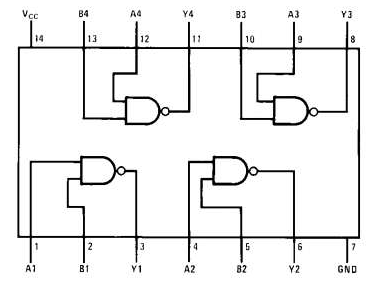
\includegraphics[width=\maxwidth{.95\linewidth}]{gfx/50_7400}
	\label{fig:50_7400}
\end{figure}


\section{7402: Quad 2-Input NOR Gate}

\section{7404: Hex Inverter}

\section{7408: Quad 2-Input AND Gate}

\section{7410: Triple 3-Input NAND Gate}

\section{7411: Triple 3-Input AND Gate}

\section{7413: Dual 4-Input NAND Gate (Schmitt-trigger)}

\section{7414: Hex Inverter (Schmitt-trigger)}

\section{7418: Dual 4-Input NAND Gate (Schmitt-trigger Inputs)}

\section{7419: Hex Inverter (Schmitt-trigger Inputs)}

\section{7420: Dual 4-Input NAND Gate}

\section{7421: Dual 4-Input AND Gate}

\section{7424: Quad 2-Input NAND Gate (Schmitt-trigger)}

\section{7427: Triple 3-Input NOR Gate}

\section{7430: Single 8-Input NAND Gate}

\section{7432: Quad 2-Input OR Gate}

\section{7436: Quad 2-Input NOR Gate}

\section{7442: BCD to Decimal Decoder}

\section{7443: Excess-3 to Decimal Decoder}

\section{7444: Gray to Decimal Decoder}

\section{7447: BCD to 7-Segment Decoder}

\section{7451: Dual AND-OR-INVERT Gate}

\section{7454: Four-wide AND-OR-INVERT Gate}

\section{7458: Dual AND-OR Gate}

\section{7464: 4-2-3-2 AND-OR-INVERT Gate}

\section{7474: Dual D-Flipflops with Preset and Clear}

\section{7485: 4-Bit Magnitude Comparator}

\section{7486: Quad 2-Input XOR Gate}

\section{74125: Quad Bus Buffer, 3-State Outputs, Neg Enable}

\section{74165: 8-Bit Parallel-to-Serial Shift Register}

\section{74175: Quad D-Flipflop, Asynchronous Reset}

\section{74266: Quad 2-Input XNOR Gate}

\section{74273: Octal D-Flipflop with Clear}

\section{74283: 4-Bit Binary Full Adder}

\section{74377: Octal D-Flipflop with Enable}



%*******************************************************
% New Appendix Here
%*******************************************************
%\chapter{New Appendix Here}
%\label{ap:ch:new_appendix_here}
